\documentclass{sig-alternate-05-2015}

\usepackage{xcolor}
\usepackage{pifont}
\newcommand{\quadrat}{\ding{110}}%


\begin{document}

% Copyright
\setcopyright{acmcopyright}
%\setcopyright{acmlicensed}
%\setcopyright{rightsretained}
%\setcopyright{usgov}
%\setcopyright{usgovmixed}
%\setcopyright{cagov}
%\setcopyright{cagovmixed}


% DOI
%\doi{10.475/123_4}

% ISBN
%\isbn{123-4567-24-567/08/06}

%Conference
\conferenceinfo{ACM SigSpatial '16}{October 31 - Thursday November 3, 2016, San Francisco Bay Area, California, USA}

%\acmPrice{\$15.00}

%
% --- Author Metadata here ---
%\conferenceinfo{WOODSTOCK}{'97 El Paso, Texas USA}
%\CopyrightYear{2007} % Allows default copyright year (20XX) to be over-ridden - IF NEED BE.
%\crdata{0-12345-67-8/90/01}  % Allows default copyright data (0-89791-88-6/97/05) to be over-ridden - IF NEED BE.
% --- End of Author Metadata ---

\title{BigGIS: A Predictive and Prescriptive Geographic Information System based on High-Dimensional Geo-Temporal Data Structures ("Vision Paper")\titlenote{(Produces the permission block, and
copyright information). For use with
SIG-ALTERNATE.CLS. Supported by ACM.}}
\subtitle{[Extended Abstract]
\titlenote{A full version of this paper is available as
\textit{Author's Guide to Preparing ACM SIG Proceedings Using
\LaTeX$2_\epsilon$\ and BibTeX} at
\texttt{www.acm.org/eaddress.htm}}}
%
% You need the command \numberofauthors to handle the 'placement
% and alignment' of the authors beneath the title.
%
% For aesthetic reasons, we recommend 'three authors at a time'
% i.e. three 'name/affiliation blocks' be placed beneath the title.
%
% NOTE: You are NOT restricted in how many 'rows' of
% "name/affiliations" may appear. We just ask that you restrict
% the number of 'columns' to three.
%
% Because of the available 'opening page real-estate'
% we ask you to refrain from putting more than six authors
% (two rows with three columns) beneath the article title.
% More than six makes the first-page appear very cluttered indeed.
%
% Use the \alignauthor commands to handle the names
% and affiliations for an 'aesthetic maximum' of six authors.
% Add names, affiliations, addresses for
% the seventh etc. author(s) as the argument for the
% \additionalauthors command.
% These 'additional authors' will be output/set for you
% without further effort on your part as the last section in
% the body of your article BEFORE References or any Appendices.

\numberofauthors{3} %  in this sample file, there are a *total*
% of EIGHT authors. SIX appear on the 'first-page' (for formatting
% reasons) and the remaining two appear in the \additionalauthors section.
%
\author{
% You can go ahead and credit any number of authors here,
% e.g. one 'row of three' or two rows (consisting of one row of three
% and a second row of one, two or three).
%
% The command \alignauthor (no curly braces needed) should
% precede each author name, affiliation/snail-mail address and
% e-mail address. Additionally, tag each line of
% affiliation/address with \affaddr, and tag the
% e-mail address with \email.
%
% 1st. author
\alignauthor
Firstname Lastname\titlenote{Lorem Ipsum}\\
       \affaddr{University of Applied Sciences Karlsruhe}\\
       \affaddr{Moltkestr. 30}\\
       \affaddr{Karlsruhe, Germany}\\
       \email{vorname.nachname@hs-karlsruhe.de}
% 2nd. author
\alignauthor
Firstname Lastname\titlenote{Lorem Ipsum}\\
       \affaddr{University of Applied Sciences Karlsruhe}\\
       \affaddr{Moltkestrasse 30}\\
       \affaddr{Karlsruhe, Germany}\\
       \email{vorname.nachname@hs-karlsruhe.de}
% 3rd. author
\alignauthor
Firstname Lastname\titlenote{Lorem Ipsum}\\
       \affaddr{FZI Research Center for Information Technology}\\
       \affaddr{Haid-und-Neu-Str. 10-14}\\
       \affaddr{Karlsruhe, Germany}\\
       \email{nachname@fzi.de}
\and  % use '\and' if you need 'another row' of author names
% 4th. author
\alignauthor
Firstname Lastname\titlenote{Lorem Ipsum}\\
       \affaddr{FZI Research Center for Information Technology}\\
       \affaddr{Haid-und-Neu-Str. 10-14}\\
       \affaddr{Karlsruhe, Germany}\\
       \email{nachname@fzi.de}
%% 5th. author
\alignauthor
Firstname Lastname\titlenote{Lorem Ipsum}\\
       \affaddr{Data Analysis and Visualization Group}\\
       \affaddr{University of Konstanz}\\
       \affaddr{Konstanz, Germany}\\
       \email{vorname.nachname@uni-konstanz.de}
%% 6th. author
\alignauthor
Firstname Lastname\titlenote{Lorem Ipsum}\\
       \affaddr{Data Analysis and Visualization Group}\\
       \affaddr{University of Konstanz}\\
       \affaddr{Karlsruhe, Germany}\\
       \email{firstname.lastname@uni-konstanz.de}
}
% There's nothing stopping you putting the seventh, eighth, etc.
% author on the opening page (as the 'third row') but we ask,
% for aesthetic reasons that you place these 'additional authors'
% in the \additional authors block, viz.
%\additionalauthors{Additional authors: John Smith (The Th{\o}rv{\"a}ld Group,
%email: {\texttt{jsmith@affiliation.org}}) and Julius P.~Kumquat
%(The Kumquat Consortium, email: {\texttt{jpkumquat@consortium.net}}).}
%\date{30 July 1999}
% Just remember to make sure that the TOTAL number of authors
% is the number that will appear on the first page PLUS the
% number that will appear in the \additionalauthors section.

\maketitle
\begin{abstract}
%Geospatial data has always been Big Data. However today's geographic information systems reach their limits due to rapidly growing geo-related data volumes. Especially in real-time processing, these systems do not provide a sufficient design. New technologies and architectures are emerging from the context of Big Data and gain increasing importance.
\end{abstract}


%
% The code below should be generated by the tool at
% http://dl.acm.org/ccs.cfm
% Please copy and paste the code instead of the example below. 
%
%\begin{CCSXML}
%<ccs2012>
% <concept>
%  <concept_id>10010520.10010553.10010562</concept_id>
%  <concept_desc>Computer systems organization~Embedded systems</concept_desc>
%  <concept_significance>500</concept_significance>
% </concept>
% <concept>
%  <concept_id>10010520.10010575.10010755</concept_id>
%  <concept_desc>Computer systems organization~Redundancy</concept_desc>
%  <concept_significance>300</concept_significance>
% </concept>
% <concept>
%  <concept_id>10010520.10010553.10010554</concept_id>
%  <concept_desc>Computer systems organization~Robotics</concept_desc>
%  <concept_significance>100</concept_significance>
% </concept>
% <concept>
%  <concept_id>10003033.10003083.10003095</concept_id>
%  <concept_desc>Networks~Network reliability</concept_desc>
%  <concept_significance>100</concept_significance>
% </concept>
%</ccs2012>  
%\end{CCSXML}
%
%\ccsdesc[500]{Computer systems organization~Embedded systems}
%\ccsdesc[300]{Computer systems organization~Redundancy}
%\ccsdesc{Computer systems organization~Robotics}
%\ccsdesc[100]{Networks~Network reliability}


%
% End generated code
%

%
%  Use this command to print the description
%
%\printccsdesc

% We no longer use \terms command
%\terms{Theory}

\keywords{keyword1; keyword2; keyword3}

\section{Introduction}
\begin{itemize}
	\item Central role of GIS (long been used for geospatial data analyses and visualization to support decision making process)
	\item Increasing availability of various existing and new data sources (e.g. remote sensing, participatory sensing, social media, etc.) lead to a rapidly growing amount of data (volume) at varying speed (velocity) and heterogeneous structure (variety)
	\item Big data related characteristics/dimensions (V's)
	\item Evolution of GIS are (tightly) coupled with the arise of new technological and analytical approaches in computer sciences \cite{Peng2014}
	\item In the era of Big Data, arising paradigms, technologies and holistic architectural designs are gradually extending their scope enabling GIS to deal with Big Data induced requirements.
	\item Data is concrete but is often systematically biased, Reasoning about data (semantics and human-interaction), data-informed vs. data-driven?? delegating your decision-making to only what you can measure right now often de-prioritizes more important macro aspects of the problem %\url{http://andrewchen.co/know-the-difference-between-data-informed-and-versus-data-driven/}
	\item Current approaches: either exclusively archival and historical data or try to integrate real-time data source to operate on geospatial data streams (see PlanetSense) both unidirectional processing pipelines or workflows that do not leverage human experts domain knowledge and semantics to support the analytical process 
	\item \textcolor{red}{Knowledge generation is one important research area where Visual Analytics is of great use~\cite{keim2010mastering}, especially when considering uncertainty of heterogeneous data from various data sources (TODO cite paper from Hansi Senaratne from the group of Prof. Keim, either here or related work chapter). The adequate support of diverse users is another field of research where Visual Analytics methods are beneficial.}
	\item \textcolor{red}{Analyses are often performed in a descriptive, predictive or prescriptive way. While the descriptive analysis visualizes the status quo, predictive and prescriptive analysis focuses on future-oriented planning. 	As a result the underlying model and the visualization have to be tightly coupled in order for users to gain knowledge. Users have the possibility to interactively alter a model's parameters according to their knowledge, consequently the visualization adjusts to the model in a feedback-loop.}
	\item The novelity \textcolor{red}{(Our contribution)} lies in (1) an \textit{integrated analytical approach} which includes (2) \textit{human-related knowledge extraction} and (3) \textit{semantic reasoning} to process large and heterogeneous spatio-temporal data at rest and in motion, that are unstructured and from unreliable sources
	\item bridging the usability gap (source:??) between domain experts, end users and technology experts
	\item System provides predictive, prescriptive and visual tools
	\item \textcolor{red}{In the end of the introduction chapter, we should clearly formulate how we contribute to the community. This strengthens our paper and shows the reviewer our potential. Maybe this can already be done by the point above.}
\end{itemize}




\section{Related Work and Influences}

\begin{itemize}
	\item Big Data architectures: Lambda architecture \cite{Marz2014}, Kappa architecture \cite{Kreps2014}
	\item Analytics (Processing Magic):
	\item Semantics: Congintive Apps, Linked APIs
	\item Visual Analytics: Knowledge generation Model for Visual Analytics \cite{SSS+14a}
	\item \textcolor{red}{Is there a limitation with respect to the number of references we should mention here?}
\end{itemize}

\section{BigGIS Platform}

\subsection{Motivation}

\begin{itemize}
	\item cognitive biases are tendencies to think in certain ways that can lead to systematic deviations from a standard of rationality or good judgment \url{https://en.wikipedia.org/wiki/List_of_cognitive_biases}
	\item decision fatigue refers to the deteriorating quality of decisions made by an individual, after a long session of decision making \url{https://en.wikipedia.org/wiki/Decision_fatigue}
	\item \textcolor{red}{We would recommend not to have a motivation subsection here. If there is a need for a motivation of some of the aspects introduced in this chapter, it should be placed in the Introduction of Chapter 1}
\end{itemize}

\subsection{Continuous Refinement Model for BigGIS}

\begin{figure*}
\centering
	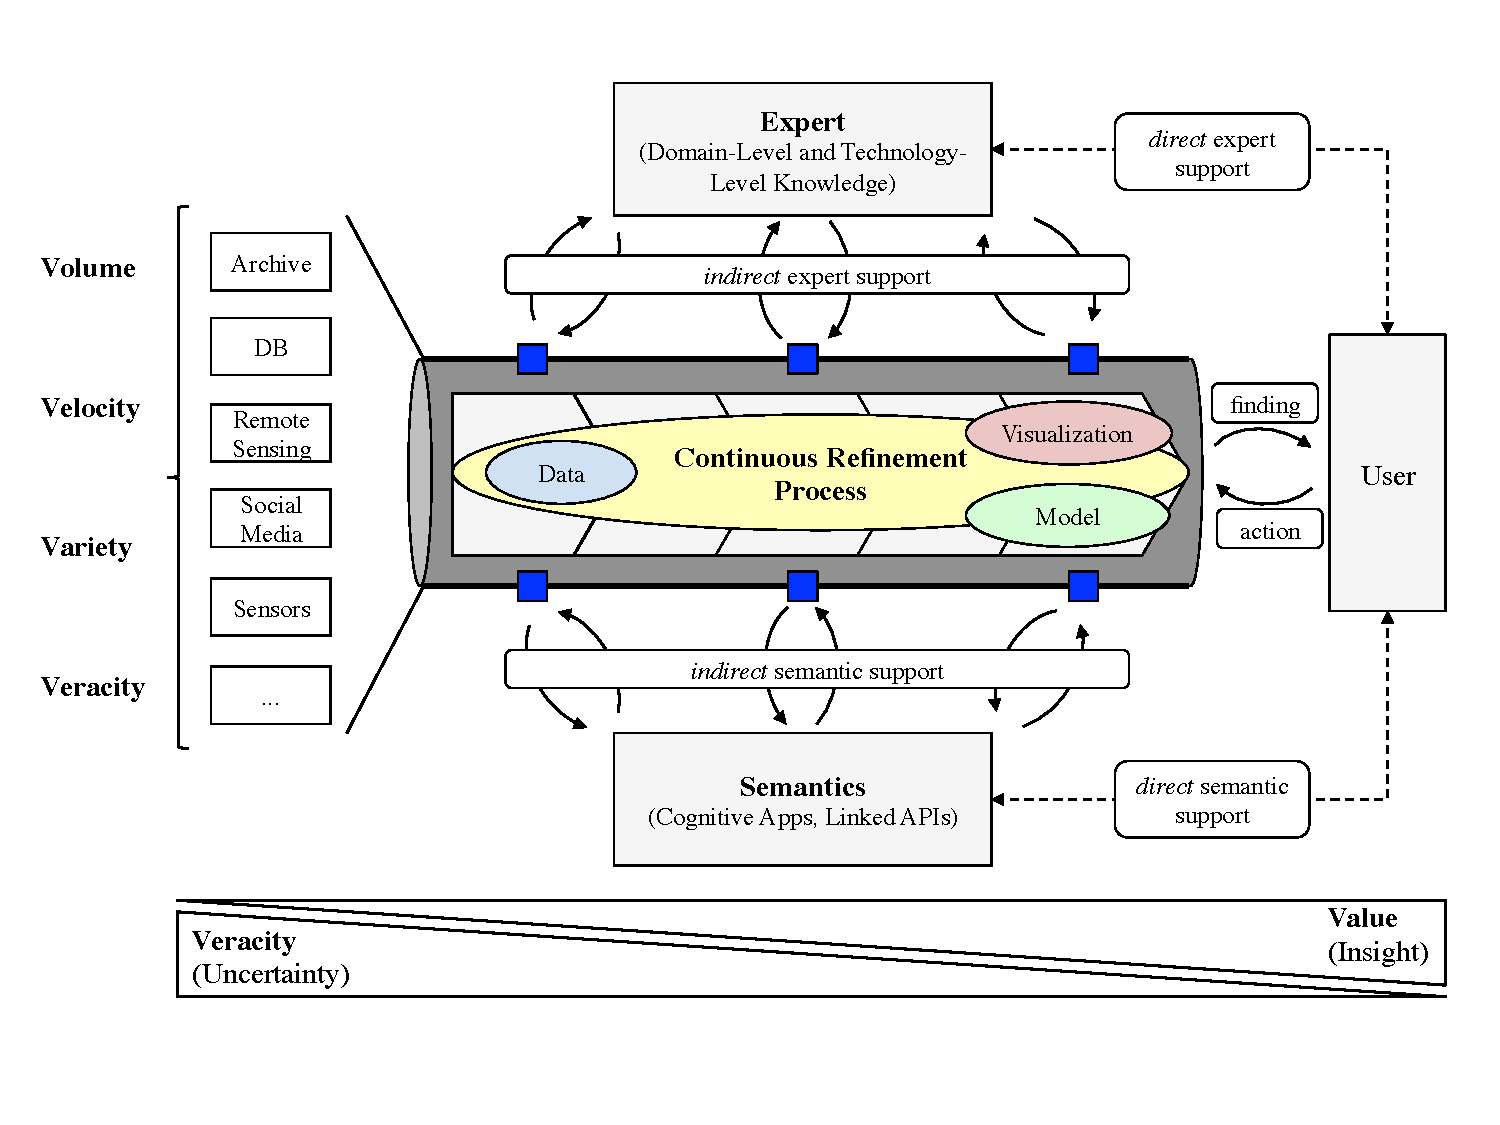
\includegraphics[width=\textwidth]{figures/biggis-workflow}
	\caption{Generic integrated analytical pipeline approach of BigGIS platform showing general purpose Continuous Refinement Process. Overcoming the usability gap between raw data and feature extraction (information gain, insight) and handling uncertainty in acquired data through indirect and direct semantic-level and expert-level support leveraged by the Knowledge Generation Model for Visual Analytics is one main contribution of BigGIS. Indirect support results from defined Refinement Gates (R-Gates \textcolor{blue}{\quadrat}).}
	\label{fig:biggisworkflow}
\end{figure*}

\begin{itemize}
	\item defining the Continuous Refinement Process (CRP), with so called R-Gates (Refinement Gates: dedicated access points, entry points)
	\item High-Level description of end-to-end workflow
	\item What is the usability gap?
	\item bridging the usability gap (source:??) between domain experts, end users and technology experts
	\item \textcolor{red}{Clearly show (also with examples) how the CRP works with respect to Visual Analytics. }
\end{itemize}

%\subsubsection{Semantics-Level}
%
%\begin{itemize}
%	\item direct semantic support
%	\item indirect semantic support
%\end{itemize}
%
%\subsubsection{Domain-Level}
%\begin{itemize}
%	\item direct domain knowledge support
%	\item indirect domain knowledge support
%\end{itemize}
%
%\subsubsection{Technology-Level}
%\begin{itemize}
%	\item direct technology knowledge support
%	\item indirect technology knowledge support
%\end{itemize}

\subsection{Architecture}

\begin{itemize}
	\item \textcolor{red}{If we talk about the architecture of a system designed according to our proposed approach, it should be on an abstract higher level. Maybe also another subsection title could be a good idea.}
\end{itemize}

\section{Scenarios}

\begin{itemize}
	\item \textcolor{red}{chapter really needed? Maybe call it "Use Cases" and say that these use cases can only be solved because WE defined this BigGIS-pipeline which is now of great help for this and that analytical task. Again, abstraction is the key here.}
	\item \textcolor{red}{This could also be a good idea when we can not show an evaluation of our proposed idea.}
\end{itemize}

\section{Conclusions and Future Work}

\begin{itemize}
	\item \textcolor{red}{Maybe call it "Discussion \& Conclusion". In the discussion part we discuss the advantages and disadvantages of our approach. In the conclusion we again shortly summarize in our own words what we just presented and give insight about future work.}
\end{itemize}

%\end{document}  % This is where a 'short' article might terminate

%ACKNOWLEDGMENTS are optional
\section{Acknowledgements}


%
% The following two commands are all you need in the
% initial runs of your .tex file to
% produce the bibliography for the citations in your paper.
\bibliographystyle{abbrv}
\bibliography{biggis-paper}  % sigproc.bib is the name of the Bibliography in this case
% You must have a proper ".bib" file
%  and remember to run:
% latex bibtex latex latex
% to resolve all references
%
% ACM needs 'a single self-contained file'!
%
%APPENDICES are optional
%\balancecolumns
%\appendix
%Appendix A


\end{document}
